\documentclass[12pt]{article}

\usepackage[brazilian]{babel}
\usepackage[utf8]{inputenc}
\usepackage[T1]{fontenc}
\usepackage{amssymb}
\usepackage{setspace}
\usepackage{lineno}
\usepackage{abntex2cite}
% Macro com novos comandos

% pacotes
\usepackage{amssymb}
\usepackage{amsmath}
\usepackage[OT2,T1]{fontenc}
\DeclareSymbolFont{cyrletters}{OT2}{wncyr}{m}{n}
\DeclareMathSymbol{\Sha}{\mathalpha}{cyrletters}{"58}
\usepackage{xspace}
\usepackage{color}
\usepackage{cancel}
\usepackage{stackengine}
\usepackage{ulem}
\usepackage{enumerate}
\usepackage{mathtools}
\usepackage{tikz}
\usepackage{tikz-3dplot}
\usepackage{pgfplots}
\usepackage{xcolor}

% Criando comandos de correcao e comentarios
\newcommand{\rem}[1]{{\color{red} \sout{#1}}} % remover texto
\newcommand{\new}[1]{{\color{blue} #1}} % Incluir texto
\newcommand{\com}[1]{{\color{ao} #1}} % Incluir coment\'ario



% bibtex path
\newcommand{\mybib}{/home/daniel/Dropbox/latex/library}

%criando novas cores
\definecolor{amethyst}{rgb}{0.6, 0.4, 0.8}
\definecolor{ao}{rgb}{0.0, 0.5, 0.0}
\definecolor{tangerine}{rgb}{1.0, 0.6, 0.4}

% encurtando comandos
\newcommand{\tx}[1]{\text{#1}}
\newcommand{\tb}[1]{\textbf{#1}}
\newcommand{\ti}[1]{\textit{#1}}
%\newcommand{\Ref}[1]{(\ref{#1})}
\newcommand{\code}[1]{\begin{semiverbatim} #1 \end{semiverbatim}}
\newcommand{\mat}[1]{\mathbf{#1}}
\newcommand{\vc}[1]{\boldsymbol{#1}}


%letras gregas
\newcommand{\Aa}{\alpha}
\newcommand{\Bb}{\beta}
\newcommand{\ow}{\omega}
\newcommand{\Ow}{\Omega}
\newcommand{\sg}{\sigma}
\newcommand{\lb}{\lambda}
\newcommand{\lbx}{\lambda_x}
\newcommand{\vep}{\varepsilon}
\newcommand{\y}{\gamma}
\newcommand{\tht}{\theta}
\newcommand{\p}{\varphi}
\newcommand{\X}{\chi}
\newcommand{\phiiw}{\hat{\phi_i}}

\newcommand{\yi}{\gamma_i}
\newcommand{\Bbi}{\beta_i}

\newcommand{\DAa}{\Delta\alpha}
\newcommand{\DBb}{\Delta\beta}
\newcommand{\Drho}{\Delta\rho}
\newcommand{\Dsg}{\Delta\sigma}
\newcommand{\DT}{\Delta \tau}

%Hamiltoniana
\newcommand{\ham}{\mathcal{H}}
\newcommand{\co}{c_0}
\newcommand{\ce}{c_{\epsilon}}
\newcommand{\cdel}{c_{\delta}}
\newcommand{\nuj}{\nu_{j}}
\newcommand{\sj}{s_{j}}
% Deltas e deltas
\newcommand{\D}{\Delta}
\newcommand{\Dt}{\Delta t}
\newcommand{\Dw}{\Delta \ow}
\newcommand{\Dx}{\Delta x}
\newcommand{\Dy}{\Delta y}
\newcommand{\Dz}{\Delta z}
\newcommand{\Dr}{\Delta r}


% Caligraficas
\newcommand{\vTau}{\mathcal{T}}
\newcommand{\cC}{\mathcal{C}}
\newcommand{\cL}{\mathcal{L}}
\newcommand{\cO}{\mathcal{O}}
\newcommand{\cR}{{\cal R}}
\newcommand{\cH}{{\cal H}}
\newcommand{\FF}{\mathcal{F}}
\newcommand{\iFF}{\mathcal{F}^{-1}}

\newcommand{\cHm}[1][m]{\cH^{(#1)} }

% conjuntos
\newcommand{\F}{\mathbb{F}}
\newcommand{\R}{\mathbb{R}}
\newcommand{\I}{\mathbb{I}}
\newcommand{\C}{\mathbb{C}}
\newcommand{\Z}{\mathbb{Z}}
\newcommand{\N}{\mathbb{N}}

\newcommand{\fM}{\mathfrak{M}}

\newcommand{\M}[1][]{\mathbb{M}#1}
\newcommand{\MR}[1][\mn]{\M[#1](\R)}

%Vetores e matrizes
\newcommand{\ve}[1][i]{\boldsymbol{\hat{e}_{#1}}}

\newcommand{\matT}[1]{\mat{#1}^T}
\newcommand{\matH}[1]{\mat{#1}^{\ast}}

\newcommand{\mA}{\mat{A}}
\newcommand{\mAi}{\mA^{-1}}
\newcommand{\mAT}{\matT{A}}
\newcommand{\mAH}{\matH{A}}

\newcommand{\cofA}[2][\mA]{\Delta^{(#1)}_{#2}}
\newcommand{\cofAij}{\cofA{ij}}

\newcommand{\mB}{\mat{B}}
\newcommand{\mBi}{\mB^{-1}}
\newcommand{\mBT}{\matT{B}}
\newcommand{\mBH}{\matH{B}}

\newcommand{\mE}{\mat{E}}
\newcommand{\mH}{\mat{H}}
\newcommand{\mHX}{\mat{H}_{\X} }
\newcommand{\mHXb}{\bar{\mat{H}}_{\X} }
\newcommand{\mR}{\mat{R}}
\newcommand{\mC}{\mat{C}}
\newcommand{\mS}{\mat{S}}
\newcommand{\mX}{\mat{X}}
\newcommand{\mY}{\mat{Y}}
\newcommand{\mO}{\mat{0}}
\newcommand{\mI}{\mat{I}}
\newcommand{\mU}{\mat{U}}
\newcommand{\mV}{\mat{V}}
\newcommand{\mW}{\mat{W}}
\newcommand{\mL}{\mat{L}}
\newcommand{\mSg}{\mat{\Sigma}}
\newcommand{\hmL}{\hat{\mL}}

\newcommand{\mHm}[1][m]{\mH^{(#1)}}

\newcommand{\aij}[1][ij]{a_{#1}}
\newcommand{\bij}[1][ij]{b_{#1}}
\newcommand{\cij}[1][ij]{c_{#1}}

\newcommand{\maij}[2][ij]{\left[\aij[#1]\right]#2}
\newcommand{\mbij}[2][ij]{\left[\bij[#1]\right]#2}

\newcommand{\mn}{_{m \times n}}
\newcommand{\nn}{_{n \times n}}
\newcommand{\n}{_{n}}
\newcommand{\mxl}{_{m \times 1}}
\newcommand{\nxl}{_{n \times 1}}

\newcommand{\vi}{\,\hat{\vc{i}}}
\newcommand{\vj}{\,\hat{\vc{j}}}
\newcommand{\vk}{\,\hat{\vc{k}}}


\newcommand{\x}{\vc{x}}
\newcommand{\vu}{\vc{u}}
\newcommand{\hvu}{\hat{\vu}}
\newcommand{\vw}{\vc{w}}
\newcommand{\vx}{\vc{x}}
\newcommand{\vv}{\vc{V}}
\newcommand{\vh}{\vc{h}}
\newcommand{\vd}{\vc{d}}
\newcommand{\hvd}{\hat{\vc{d}}}
\newcommand{\vr}{\vc{r}}
\newcommand{\vf}{\vc{f}}
\newcommand{\vt}{\vc{\t}}
\newcommand{\vht}{\hat{\vc{t}}}
\newcommand{\vp}{\vc{p}}
\newcommand{\vy}{\vc{y}}
\newcommand{\vb}{\vc{b}}
\newcommand{\vhb}{\hat{\vc{b}}}
\newcommand{\va}{\vc{a}}
\newcommand{\vn}{\vc{n}}
\newcommand{\vhn}{\hat{\vc{n}}}
\newcommand{\vO}{\vc{0}}

\newcommand{\hvn}{\hat{\vn}}
\newcommand{\hvt}{\hat{\vt}}
\newcommand{\hp}{\hat{p}}
\newcommand{\hg}{\hat{g}}
\newcommand{\fw}{\skew{4.5}\hat{f}(\omega)}
\newcommand{\pxw}{\skew{4.5}\hat{P_x}}
\newcommand{\vwf}{\skew{4.5}\hat{V}}
\newcommand{\phixw}{\hat{\phi_x}}
\newcommand{\gw}{\skew{4.5}\hat{G}}
\newcommand{\Gw}{\skew{4.5}\hat{\mathcal{G}}}
\newcommand{\pw}{\skew{4.5}\hat{P}}
\newcommand{\qw}{\skew{4.5}\hat{q}(\vc{r},\ow)}
\newcommand{\ffw}{\vc{\skew{4.5}\hat{f}}(\vc{r},\ow)}

\newcommand{\vR}{\vc{R}}
\newcommand{\vF}{\vc{F}}
\newcommand{\vZ}{\vc{Z}}
\newcommand{\vY}{\vc{Y}}
\newcommand{\vW}{\vc{W}}
\newcommand{\vA}{\vc{A}}
\newcommand{\vB}{\vc{B}}
\newcommand{\vC}{\vc{C}}
\newcommand{\vD}{\vc{D}}
\newcommand{\vM}{\vc{M}}
\newcommand{\vG}{\vc{\Gamma}}
\newcommand{\vT}{\vc{\Theta}}
\newcommand{\vP}{\vc{\Phi}}


\newcommand{\m}{\vc{m}}
\newcommand{\tm}{\tilde{\vc{m}}}
\newcommand{\mz}{\m_0}
\newcommand{\mi}[1][]{\m_{i#1}}
\newcommand{\mj}{\m_j}
\newcommand{\mii}{\mi[+1]}
\newcommand{\dm}{\delta\m}
\newcommand{\dmest}{\delta m^{\est}}


\newcommand{\h}{\vc{h}}
\newcommand{\hz}{\h_0}
\newcommand{\hii}{\h_{i+1}}
\newcommand{\hi}{\h_i}
\newcommand{\hj}{\h_j}

% Funcoes
\newcommand{\ft}[1][]{f_{#1}(t)}
\newcommand{\gt}[1][]{g_{#1}(t)}
\newcommand{\hfw}[1][]{\hf_{#1}(\ow)}
\newcommand{\hhw}[1][]{\hh_{#1}(\ow)}
\newcommand{\fx}{f(x)}
\newcommand{\fxy}{f(x,y)}
\newcommand{\Pxy}{P(x,y)}
\newcommand{\Qxy}{Q(x,y)}
\newcommand{\fxyz}{f(x,y,z)}


\newcommand{\gx}{g(x)}
\newcommand{\gxy}{g(x,y)}
\newcommand{\yt}{y(t)}
\newcommand{\xt}{x(t)}
\newcommand{\yn}{y[n]}
\newcommand{\yk}{y_k}
\newcommand{\Yn}{Y_n}
\newcommand{\wN}[1][-nk]{w_N^{#1}}
\newcommand{\xn}{x[n]}
\newcommand{\mut}[1][]{\mu_{#1}(t)}
\newcommand{\mun}[1][]{\mu_{#1}[n]}
\newcommand{\hf}{\hat f}
\newcommand{\hx}{\hat x}
\newcommand{\hh}{\hat h}
\newcommand{\sgn}{\textrm{sgn} }
\newcommand{\sinc}{\textrm{sinc} }


\newcommand{\ep}[1][\ow t]{e^{i #1}}
\newcommand{\en}[1][\ow t]{e^{-i #1}}

\newcommand{\RtR}{\R \rightarrow \R}
\newcommand{\RtC}{\R \rightarrow \C}

% trigonometria
\newcommand{\sech}{\textrm{sech}}
\newcommand{\csch}{\textrm{csch}}


% Espa\c{c}os
\newcommand{\lp}[1][p]{\ell^#1}
\newcommand{\ld}{\lp[2]}

\newcommand{\Lp}[1][p]{L^#1}
\newcommand{\Ld}{\Lp[2]}

% Operadores
\renewcommand{\d}[2][]{\,\textrm{d}^{#1}#2}
\newcommand{\dx}[1][x]{\d{#1}}
\newcommand{\diiix}{\d[3]{\x}}
\newcommand{\diix}{\d[2]{\x}}
\newcommand{\dt}{\dx[t]}
\newcommand{\dr}{\dx[r]}
\newcommand{\dvr}{\dx[\vr]}
\newcommand{\ds}{\dx[s]}
\newcommand{\dtht}{\dx[\tht]}
\newcommand{\dtau}{\dx[\tau]}
\newcommand{\dy}{\dx[y]}
\newcommand{\dz}{\dx[z]}
\newcommand{\dw}{\dx[\ow]}
\newcommand{\dA}{\dx[A]}
\newcommand{\dV}{\dx[V]}
\newcommand{\dS}{\dx[S]}
\newcommand{\dvS}{\dx[\vc{S}]}

%\newcommand{\tr}{\textrm{tr}}
\newcommand{\posto}{\textrm{posto}}
\newcommand{\rank}{\textrm{rank}}
\newcommand{\nul}{\textrm{null}}
\newcommand{\im}{\textrm{Im}}
\newcommand{\re}{\textrm{Re}}


\newcommand{\dddtt}[1][]{\frac{\partial^2 #1}{\partial t^2}}
\newcommand{\dddxx}[1][]{\frac{\partial^2 #1}{\partial x^2}}
\newcommand{\dddxi}[1][]{\frac{\partial^2 #1}{\partial x_i^2}}
\newcommand{\dddzz}[1][]{\frac{\partial^2 #1}{\partial z^2}}
\newcommand{\dddyy}[1][]{\frac{\partial^2 #1}{\partial y^2}}
\newcommand{\ddd}[2][]{\frac{\partial^2 #1}{\partial #2^2}}
\newcommand{\dddc}[3][]{\frac{\partial^2 #1}{\partial #2 \partial #3}}

\newcommand{\ddy}[1][]{\frac{\partial #1}{\partial y}}
\newcommand{\ddi}[1][]{\frac{\partial #1}{\partial i}}
\newcommand{\ddz}[1][]{\frac{\partial #1}{\partial z}}
\newcommand{\ddx}[1][]{\frac{\partial #1}{\partial x}}
\newcommand{\ddt}[1][]{\frac{\partial #1}{\partial t}}
\newcommand{\dd}[2][]{\frac{\partial #1}{\partial #2}}

\newcommand{\DD}[2][]{\frac{\dx[#1]}{\dx[#2]}}
\newcommand{\DDn}[3][n]{\frac{\d[#1]#2}{\dx[#3]^{#1}}}

\newcommand{\DDx}[1][]{\frac{\dx[#1]}{\dx}}
\newcommand{\DDt}[1][]{\frac{\dx[#1]}{\dt}}
\newcommand{\DDDtt}[1][]{\frac{\dx[]^2#1}{\dt^2}}
\newcommand{\DDw}[1][]{\frac{\dx[#1]}{\dw}}


\newcommand{\lap}[1][]{\nabla^2_{#1}}
\newcommand{\Grad}[1][]{\nabla_{#1}}
\newcommand{\Div}[1][]{\nabla_{#1} \cdot }
\newcommand{\Rot}[1][]{\nabla_{#1} \times}

\newcommand{\dk}[1][]{\delta_{#1}}
\newcommand{\del}[1][t]{\delta\!\left(#1\right)}
\newcommand{\delc}[1][n]{\delta\left[#1\right]}

\newcommand{\intifif}{\int_{-\infty}^{\infty}}
\newcommand{\intOif}{\int_{0}^{\infty}}

\newcommand{\dint}{\displaystyle\int}

\newcommand{\sumifif}[1][n]{\sum_{#1=-\infty}^{\infty}}
\newcommand{\sumOif}[1][n]{\sum_{#1=0}^{\infty}}
\newcommand{\sumuif}[1][n]{\sum_{#1=1}^{\infty}}

\newcommand{\sumON}[1][k]{\sum_{#1=0}^{N-1}}

\newcommand{\norm}[2][]{\left\Vert#2\right\Vert_{#1}}
\newcommand{\mdl}[1]{\left|#1\right|}
\newcommand{\PI}[2]{\left\langle#1,#2\right\rangle}

\newcommand{\cchts}[1]{\left[#1\right]}
\newcommand{\Cchts}[1]{\left[\begin{array}#1 \end{array}\right]}
\newcommand{\prts}[1]{\left(#1\right)}
\newcommand{\chvs}[1]{\left\{#1\right\}}
\newcommand{\Chvs}[1]{\left\{\begin{array}#1 \end{array}\right\}}
\newcommand{\Sist}[1]{\left\{\begin{array}#1 \end{array}\right.}

\newcommand{\fft}[2][]{{\cal F}^{#1}\cchts{#2}}
\newcommand{\lplc}[2][]{{\cal L}^{#1}\cchts{#2}}
\newcommand{\hilb}[2][]{{\cal H}^{#1}\cchts{#2}}

% \newcommand{\mod}{\textrm{mod}}

%ondas elasticas
\newcommand{\kz}{k_z}
\newcommand{\ky}{k_y}
\newcommand{\kx}{k_x}

\newcommand{\kAa}{k_{\Aa}}
\newcommand{\kBa}{k_{\Bb}}

\newcommand{\vua}{\vu_{\Aa}}
\newcommand{\vub}{\vu_{\Bb}}

% Diferencas finitas
\newcommand{\uijn}[3][]{u_{i#1,j#2}^{n#3}}
\newcommand{\uin}[2][]{u_{i#1}^{n#2}}


\newcommand{\kij}[2][]{K_{i#1,j#2}}
\newcommand{\Pij}[3][t]{P_{i#2,j#3}(#1)}
\newcommand{\Vxij}[3][t]{V\!x_{i#2,j#3}(#1)}
\newcommand{\Vzij}[3][t]{V\!z_{i#2,j#3}(#1)}
\newcommand{\Vxijl}[3][]{V\!x_{i#1,j#2}^{l#3}(t)}
\newcommand{\Vzijl}[3][]{V\!z_{i#1,j#2}^{l#3}(t)}
\newcommand{\qij}[3][]{q_{i#2,j#3}}
\newcommand{\fxij}[2][]{fx_{i#1,j#2}}
\newcommand{\fzij}[2][]{fz_{i#1,j#2}}
\newcommand{\Rhoij}[2][]{\rho_{i#1,j#2}}
\newcommand{\Rhoxij}[2][]{\rho x_{i#1,j#2}}
\newcommand{\Rhozij}[2][]{\rho z_{i#1,j#2}}
\newcommand{\csi}{{\xi}_i}


\newcommand{\Pijl}[3][]{P_{i#1,j#2}^{l#3}}
\newcommand{\vxijl}[3][]{vx_{i#1,j#2}^{l#3}}
\newcommand{\vzijl}[3][]{vz_{i#1,j#2}^{l#3}}
\newcommand{\fxijl}[3][]{fx_{i#1,j#2}^{l#3}}
\newcommand{\fzijl}[3][]{fz_{i#1,j#2}^{l#3}}
\newcommand{\qijl}[3][]{q_{i#1,j#2}^{l#3}}


\newcommand{\Uijn}[3][]{U_{i#1,j#2}^{n#3}}
\newcommand{\Uin}[2][]{U_{i#1}^{n#2}}
\newcommand{\Un}[1][]{U^{n#1}}
\newcommand{\Ui}[1][]{U_{i#1}}

\newcommand{\odf}[2][2N]{\partial^{[#1]}_{#2}}

\newcommand{\Kij}[1][ij]{K^{#1} }
\newcommand{\hpij}[1][ij]{\hat{p}^{#1} }
\newcommand{\hqij}[1][ij]{\hat{q}^{#1} }
\newcommand{\hvxij}[1][ij]{\hat{v}_x^{#1} }
\newcommand{\hvzij}[1][ij]{\hat{v}_z^{#1} }
\newcommand{\hfxij}[1][ij]{\hat{f}_x^{#1} }
\newcommand{\hfzij}[1][ij]{\hat{f}_z^{#1} }
\newcommand{\rhoxij}[1][ij]{\rho_{(x)}^{#1} }
\newcommand{\rhozij}[1][ij]{\rho_{(z)}^{#1} }
\newcommand{\bxij}[1][ij]{b_{(x)}^{#1} }
\newcommand{\bzij}[1][ij]{b_{(z)}^{#1} }
\newcommand{\xixi}[1][i]{\xi_x^{#1}}
\newcommand{\xizj}[1][j]{\xi_z^{#1}}


% par\'agrafos especiais
\newcounter{ex}
\newcommand{\ex}[1][\theex]{\paragraph{Exerc\'icio #1}\stepcounter{ex}}

\newcounter{eg}
\newcommand{\eg}[1][\theeg]{\paragraph{Exemplo #1}\stepcounter{eg}}

\newcounter{qu}
\newcommand{\qu}[2][\thequ]{\paragraph{Quest\~ao #1 #2}\stepcounter{qu}}

% Transformada z
\newcommand{\az}{A(Z)}
\newcommand{\bz}{B(Z)}
\newcommand{\xz}{X(Z)}
\newcommand{\yz}{Y(Z)}
\newcommand{\fz}{F(Z)}
\newcommand{\wz}{W(Z)}
\newcommand{\pz}{P(Z)}

\newcommand{\baoz}{\bar A\left(\frac{1}{Z}\right)}
\newcommand{\bboz}{\bar B\left(\frac{1}{Z}\right)}
\newcommand{\bpoz}{\bar P\left(\frac{1}{Z}\right)}

% Micelanea

\newcommand{\vMb}{\bar{\vM}}
\newcommand{\vMd}{\dot{\vM}}

\newcommand{\xb}{\bar{x}}
\newcommand{\wb}{\bar{w}}
\newcommand{\wbm}{\bar{w}_m}

\newcommand{\vph}{\vc{\hat{p}}}
\newcommand{\vxi}{\vc{\xi}}

\newcommand{\matlab}{\textsc{Matlab}\xspace}
\newcommand{\latex}{\LaTeX\xspace}

\newcommand{\Pp}[1][(\x,\ow)]{P^+#1}
\newcommand{\Pn}[1][(\x,\ow)]{P^-#1}
\newcommand{\pp}[1][(\x,t)]{p^+#1}
\newcommand{\pn}[1][(\x,t)]{p^-#1}
\newcommand{\Pxw}[1][]{P_{#1}(\x,\ow)}
\newcommand{\Pxxw}[2][]{P(\x_{#1}|\x_{#2},\ow)}
\newcommand{\Gxxw}[3][]{G^{#1}(\x_{#2}|\x_{#3},\ow)}
\newcommand{\pxt}{p(\x,t)}
\newcommand{\QED}{\begin{flushright}
                   \textit{Q.E.D. ${\scriptstyle\blacksquare}$}
                  \end{flushright}
}

\newcommand{\ubar}[1]{\underset{\bar{}}{#1}}

\newcommand{\adj}{\textrm{adj}\, }

% \newcommand{\enumroman}[2][black]{\end{frame}

% \setbeamertemplate{enumerate item}{{\color{#1}\insertenumlabel}}
% #2
% \setbeamertemplate{enumerate items}[ball]
% \renewcommand{\theenumi}{\arabic{enumi}}}







%\includegraphics{Figuras/}
\RequirePackage{amsmath}
\RequirePackage{graphicx}
\RequirePackage[a4paper,top=3cm,bottom=2cm,left=3cm,right=2cm]{geometry}

%%%%%%%%%%%%%%%%%%%%%%%%%%%%%%%%%%%%%%%%%%%%%%%%% documento %%%%%%%%%%%%%%%%%%%%%%%%%%%%%%%%%%%%%%%%%%%%%%%%%%%%%%%%%%

\begin{document}
\thispagestyle{empty}

 \begin{figure}[!t]
 
  \begin{center}
   
\includegraphics[scale=0.8]{Logo_UFPA.jpg}
  \end{center}

 \end{figure}

 \begin{center}
  \large{UNIVERSIDADE FEDERAL DO PARÁ} \\ {INSTITUTO DE GEOCIÊNCIAS} \\ {PROGRAMA DE PÓS-GRADUAÇÃO EM GEOFÍSICA} \\
  \vspace{2cm}
  \large{PROFESSOR: JESSÉ CARVALHO COSTA} \\
  \vspace{2cm}
  \large{RELATÓRIO 2: DISCIPLINA TÓPICOS DE INVERSÃO} \\
  \vspace{2cm}
  \large {\bf {TÍTULO: MÉTODOS DE OTIMIZAÇÃO}} \\
  \vspace{2cm}
  \large {ALUNOS: FELIPE  LOUZEIRO, LUCAS DE CASTRO COSTA, MURILLO NASCIMENTO E THYERRE AUGUSTO CARDOSO SAMPAIO} \\
  \vfill 
  \large Belém \\ 2022
 \end{center}

 
 \newpage
 \tableofcontents{}
 
 \newpage
 \setcounter{page}{1}

\section{OBJETIVOS}
 
 
\ \ \ \ \ O objetivo deste relatório é mostrar a eficácia dos métodos de otimização de primeira e segunda ordem, apresentando testes e alterações notáveis. Será analisado quantas iterações serão necessárias para cada método.
 
 
 
\section{METODOLOGIA}
\ \ \ \ \ Para a análise dos algoritmos de otimização, foram divididos testes analisando funções e linha de busca para cada método \cite{kochenderfer2019algorithms}. Para os experimentos, serão utilizados três tipos de linhas de busca.
\subsection{LINHAS DE BUSCA}
Supondo que escolhemos uma direção de descida \textit{d}, é necessário escolher
o fator de passo $\alpha$ para obter nosso próximo ponto de projeto. Uma abordagem é usar a pesquisa de linha,
que seleciona o fator de passo que minimiza a função unidimensional:
\begin{equation}
\text{minimize}_{\alpha} f(\vc{x} - \alpha \vc{d}).
\end{equation}

 A linha de busca é usada para a minimizar uma função a partir de uma direção de descida. Podemos aplicar o busca de linha da nossa escolha. Para informar o que se busca, podemos usar a derivada do objetivo de busca de linha, que é simplesmente o derivada direcional ao longo de $d$ em $\vc{x} - \alpha \vc{d}$.

Para aproximar melhor e ter menos iterações, são utilizadas condições aplicadas nas linhas de busca. Uma dessas é a de diminuição suficiente, representada por:
\begin{equation}
f(\vc{x}^{(k+1)}) \leq f(\vc{x}^{(k)}) + \beta\alpha \nabla_{\vc{d}^{(k)}}f(\vc{x}^{(k)}),
\end{equation}
sendo $\beta \in [0,1]$, nos nossos testes será utilizado $\beta  = 1 \times 10^{-4}$. Esta condição também é conhecida como condição de Armijo. 

Outra condição que foi utilizada será a de forte curvatura, representada por:
\begin{equation}
|\nabla_{\vc{d}^{(k)}}f(\vc{x}^{(k+1)})| \leq  - \sigma \nabla_{\vc{d}^{(k)}}f(\vc{x}^{(k)})
\end{equation}
no qual $\sigma$ controla quão superficial deve ser a próxima derivada direcional.

Juntando as duas condições ditas, formam as condições fortes de Wolfe, sendo a de Armijo a primeira, enquanto a de forte curvatura a segunda.

Nos nossos testes, serão utilizadas duas linhas de busca: a primeira sem considerar condições, a busca simples, e a segunda  utilizando as condições fortes de \textit{Wolfe}.
 



\subsection{FUNÇÕES}
Para os testes dos métodos de otimização, serão utilizadas funções com o intuito de analisar a quantidade de iterações necessárias. Uma das funções utilizadas foi:
\begin{equation}
f(\vc{x}) = 3(x_1)^2 + 24(x_2)^2 \label{eq1}
\end{equation}

Outra das funções que será usada é a de \textit{Rosenbrock} para 6 componentes, como apresentada abaixo:
\begin{eqnarray}
f(\vc{x}) &=& b(x_2 - x_1^2)^2+ (a - x_1)^2 + b(x_3 - x_2^2)^2 + (a-x_2)^2 
+ b(x_4 - x_3^2)^2+ (a - x_3)^2 \nonumber\\
&&+ b(x_5 - x_1^4)^2+ (a - x_4)^2 + b(x_6 - x_1^5)^2+ (a - x_5)^2, \label{eq2}
\end{eqnarray}
sendo $a$ e $b$ parâmetros da função definidos como $1$ e $5$, respectivamente.
 
 \section{MÉTODOS DE OTIMIZAÇÃO}
 Nesta seção, serão avaliados quantas iterações foram necessárias e em cada linha de busca, para saber quais são mais eficazes nas funções apresentadas. Esses testes serão feitos a partir das Equações \ref{eq1} e \ref{eq2}, para facilitar, serão chamadas de primeira e segunda função, respectivamente. Nas duas funções, foram feitos testes com duas linhas de busca: a simples e a com as condições fortes de Wolf. 
\subsection{MÉTODOS DE PRIMEIRA ORDEM}
\subsubsection{\textit{STEEPEST DESCENT}}
Neste método, foi utilizado o máximo de 5000 iterações. Para a primeira função, os resultados são apresentados nas Figuras \ref{fig:steep1f} e \ref{fig:steep2f}. Para a busca com linha simples foram necessárias 966 iterações para chegar próximo do resultado, enquanto que para as condições fortes de Wolf foram 1068 iterações.
\begin{figure}[ht!]
	\centering
	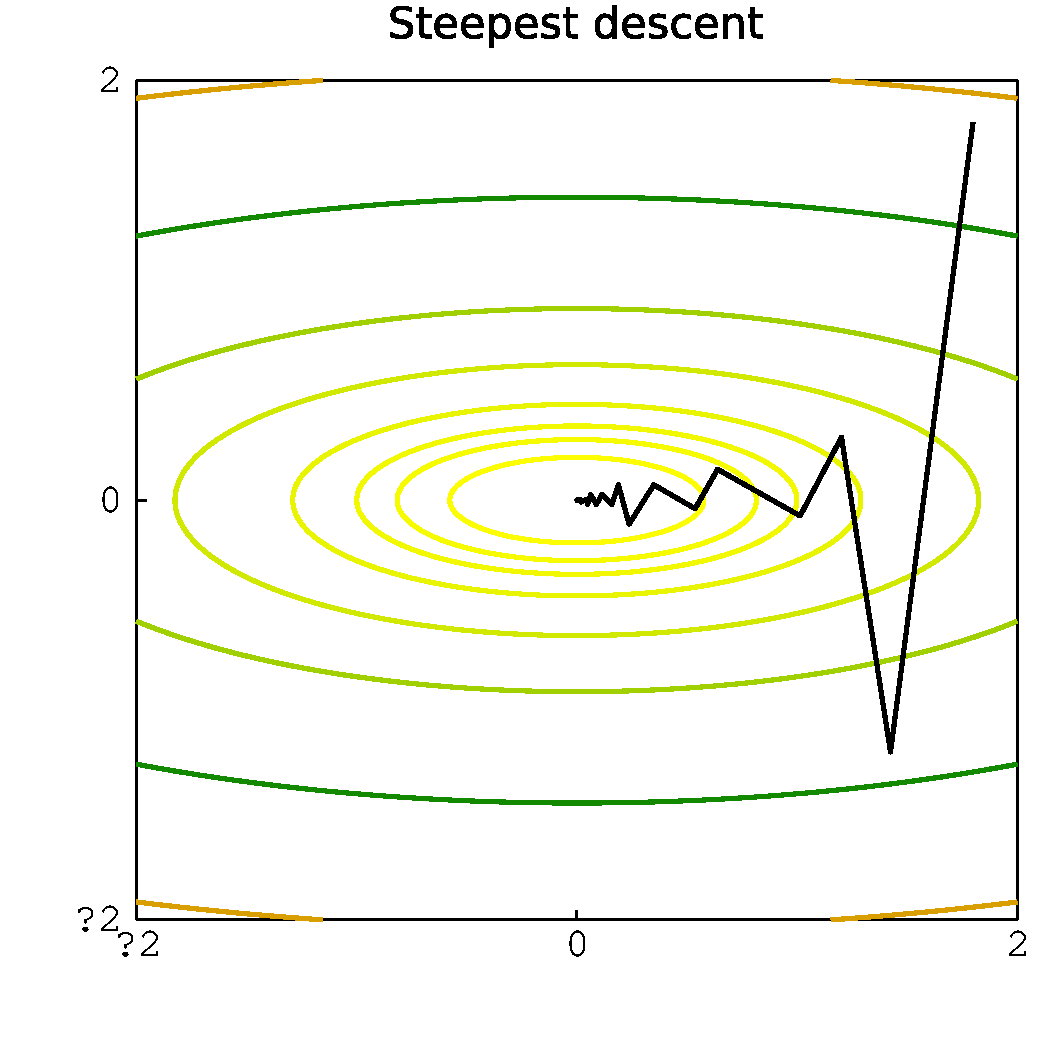
\includegraphics[width=10cm]{Figuras/Steepest_descent_linef2}
		\caption{Método de otimização \textit{steepest descent} para a primeira função. Utilizada a linha de busca simples. Nesta função de duas dimensões, o ponto
			inicial é [1.8, 1.8] e o ponto mínimo [0, 0]. Esse padrão será adotado para todos os casos da primeira função.} 
	\label{fig:steep1f}
\end{figure} 
\begin{figure}[ht!]
	\centering
	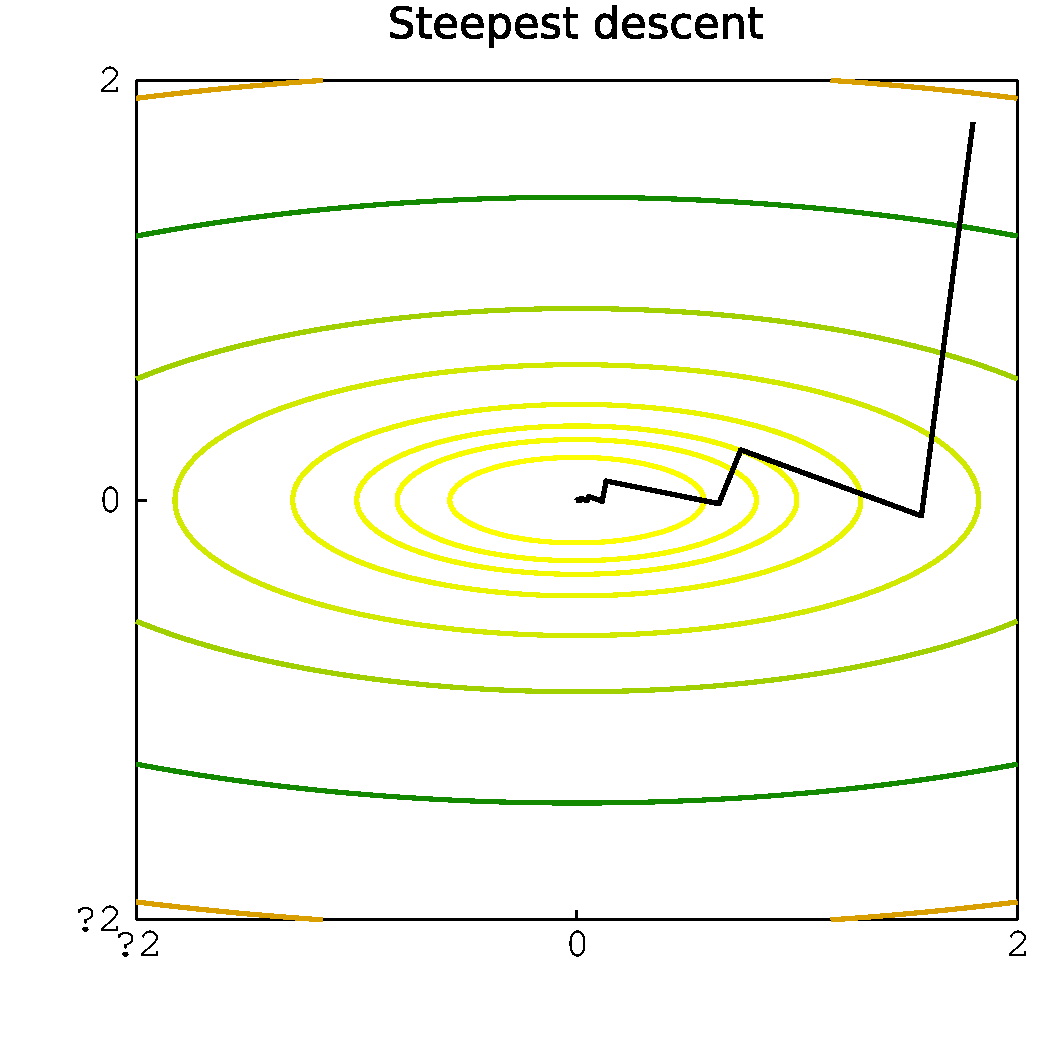
\includegraphics[width=10cm]{Figuras/Steepest_descent_wolff2}
		\caption{Método de otimização \textit{steepest descent} para a primeira função. Utilizada a linha de busca com as condições fortes de Wolf.} 
	\label{fig:steep2f}
\end{figure} 

Para a segunda função, os resultados gráficos são apresentados nas Figuras \ref{fig:steep1} e \ref{fig:steep3}. Para a linha de busca simples, foram necessárias 2042 iterações, enquanto para as condições fortes de Wolf foram feitas 1144 para atingir próximo do mínimo. 
\begin{figure}[ht!]
	\centering
	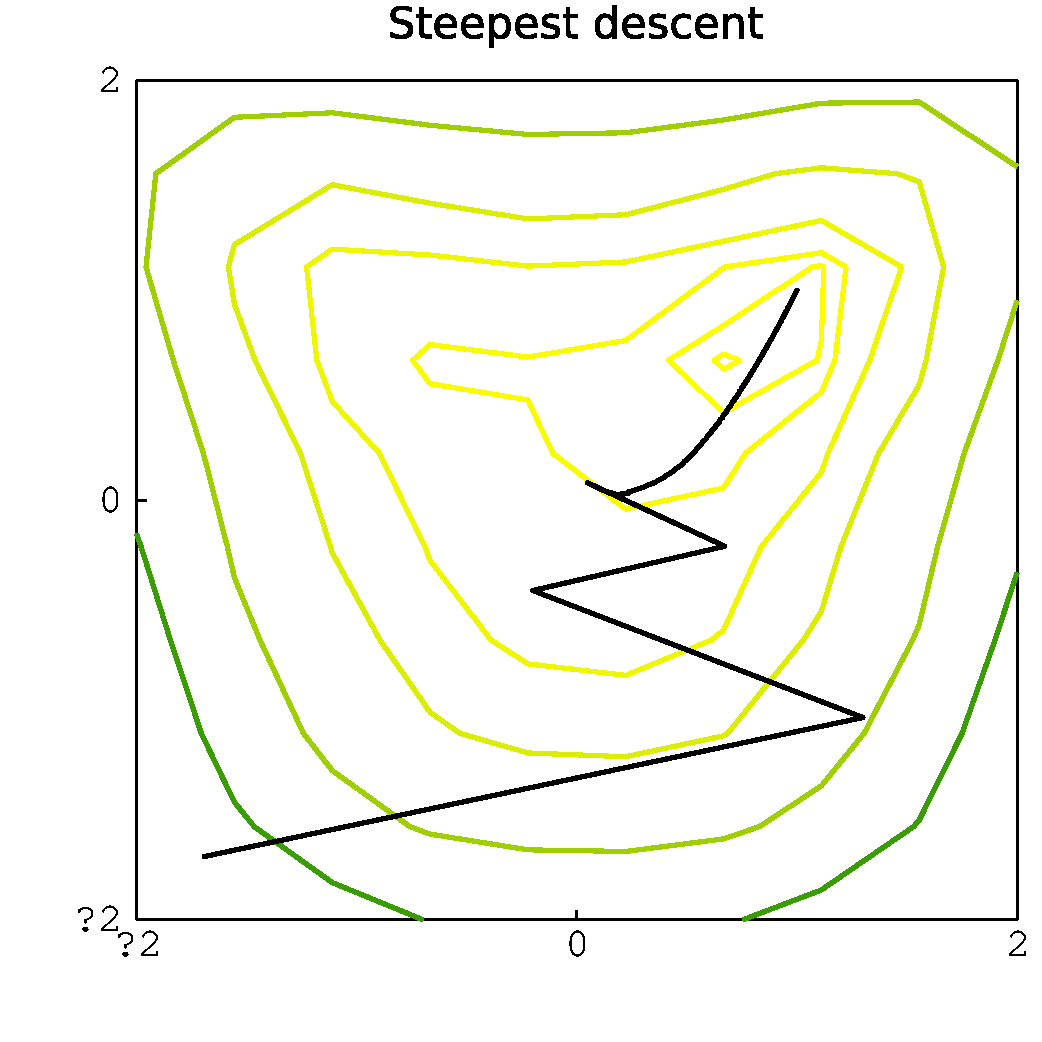
\includegraphics[width=10cm]{Figuras/Steepest_descent_linef1}
	\caption{Método de otimização \textit{steepest descent} para a segunda função. Utilizada a linha de busca simples. Neste corte de função de seis	dimensões, o ponto inicial $[-1.7, -1.7, -1.7, -1.7, -1.7, -1.7]$ e o ponto mínimo $[1.0, 1.0, 1.0, 1.0, 1.0, 1.0]$. Este padrão será mantido para todos os casos da segunda função.} 
	\label{fig:steep1}
\end{figure} 
\begin{figure}[ht!]
	\centering
	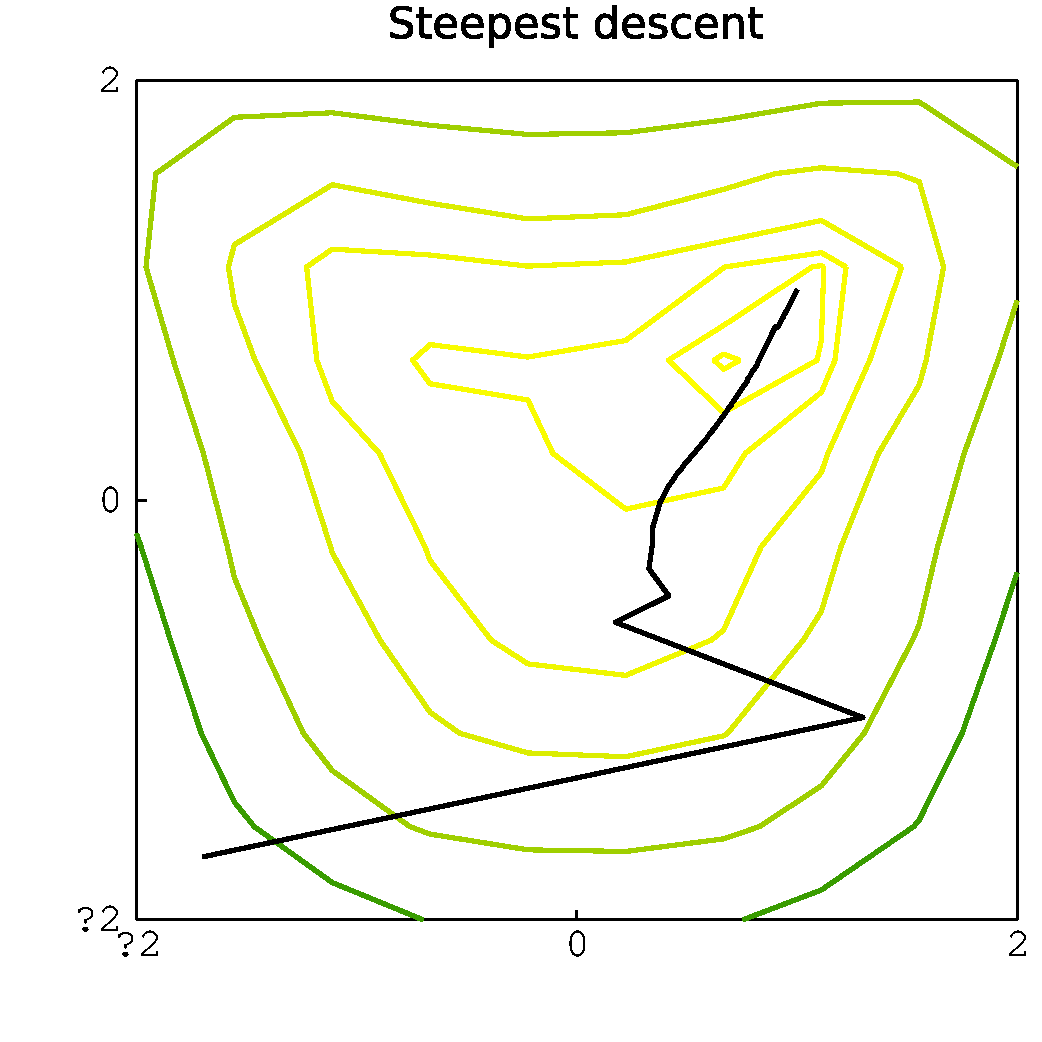
\includegraphics[width=10cm]{Figuras/Steepest_descent_strongf1}
	\caption{Método de otimização \textit{steepest descent} para a segunda função. Utilizada a linha de busca com as condições fortes de Wolf.}
	\label{fig:steep3}
\end{figure}


\subsubsection{\textit{CONJUGATE GRADIENT DESCENT}}
Neste método, foram repetidas o máximo de 5000 iterações do caso anterior. Nas Figuras \ref{fig:conj1f} e \ref{fig:conj2f} estão representadas o método aplicado para a primeira função. Para a busca de linha simples, foram utilizadas 2459 iterações, enquanto que para o de condições de Wolf foram 152.
\begin{figure}[ht!]
	\centering
	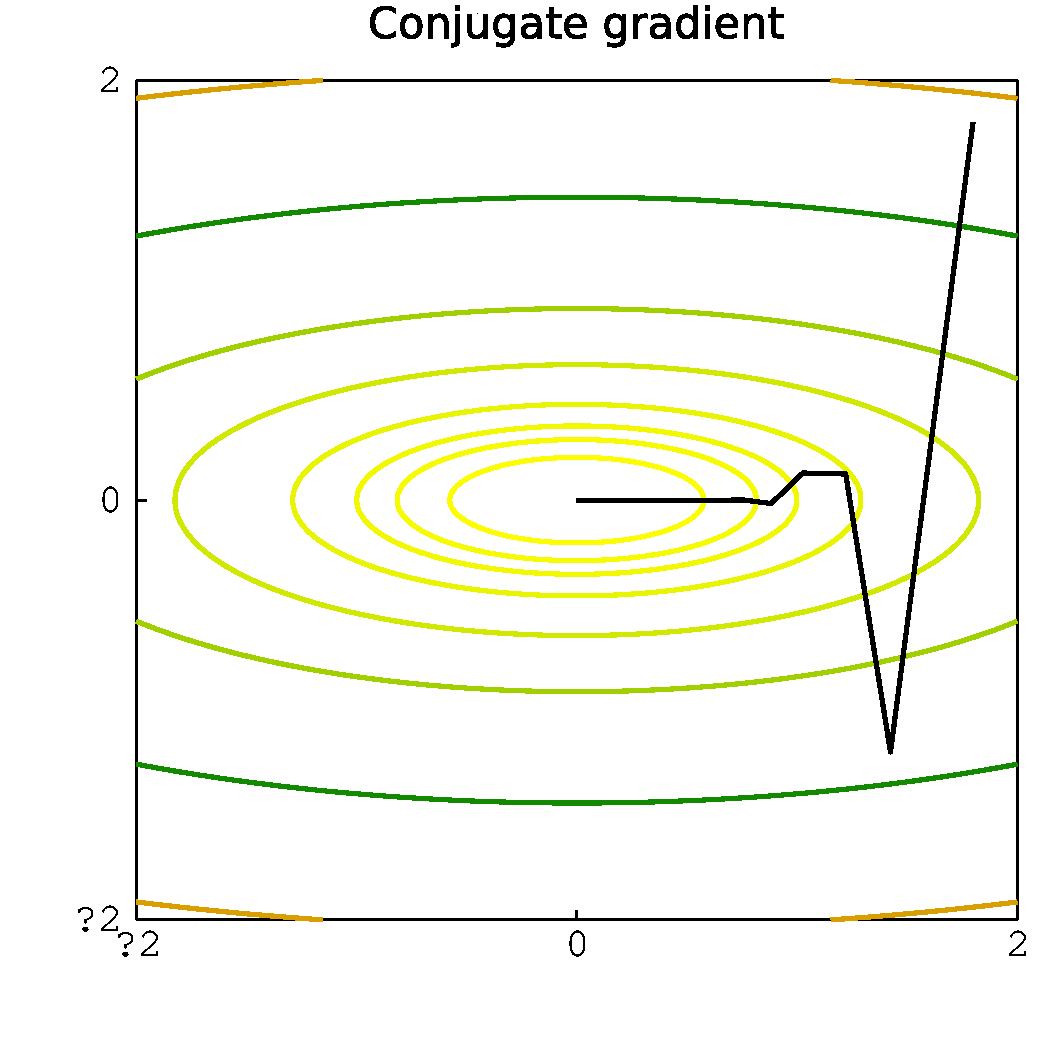
\includegraphics[width=10cm]{Figuras/Conjugate_gradient_linef2}
	\caption{Método de otimização \textit{conjugate gradient descent} para a primeira função. Utilizada a linha de busca simples.}
	\label{fig:conj1f}
\end{figure} 
\begin{figure}[ht!]
	\centering
	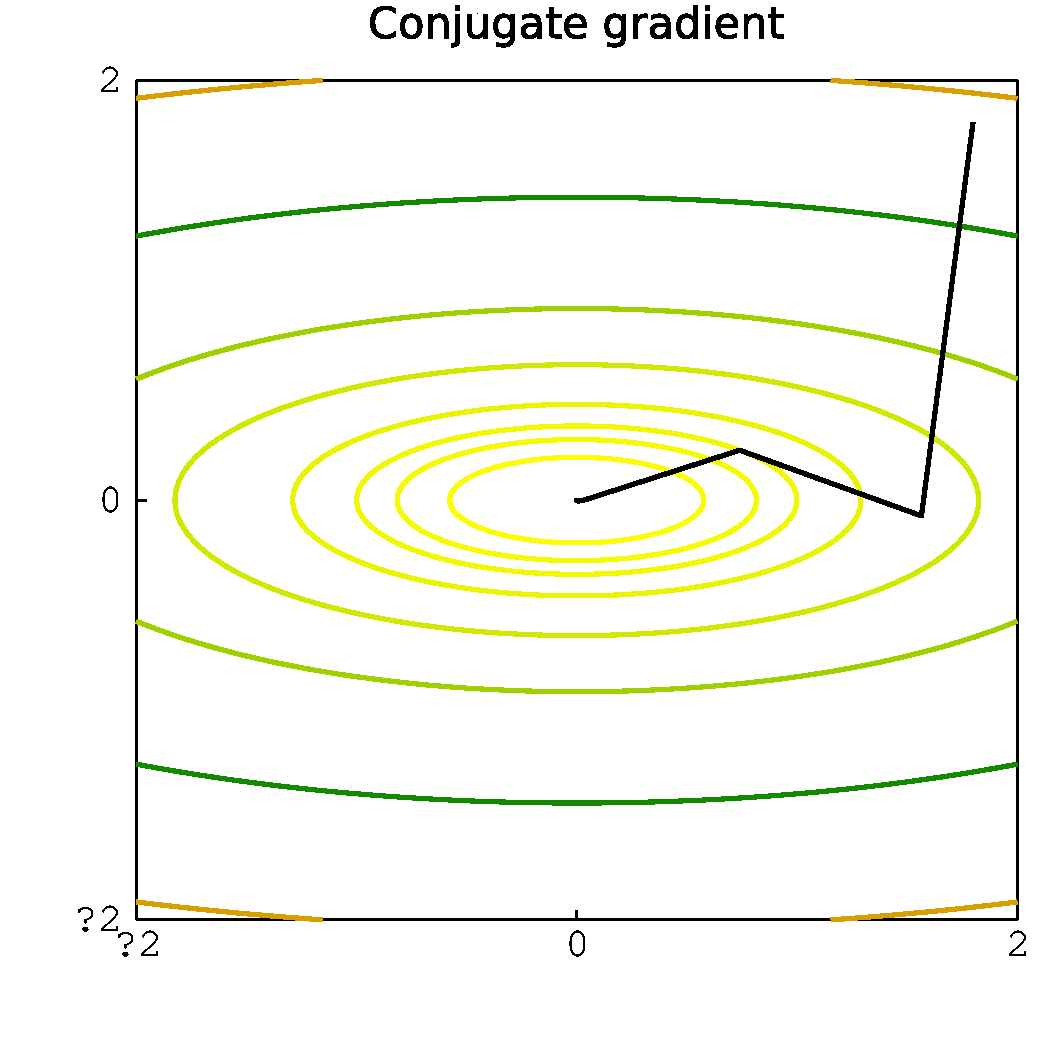
\includegraphics[width=10cm]{Figuras/Conjugate_gradient_wolff2}
	\caption{Método de otimização \textit{conjugate gradient descent} para a primeira função. Utilizada a linha de busca com as condições fortes de Wolf.}
	\label{fig:conj2f}
\end{figure} 

Para a segunda função, o de busca de linha simples foram necessárias 2783 iterações, enquanto para as condições fortes de Wolf foram 105.
\begin{figure}[ht!]
	\centering
	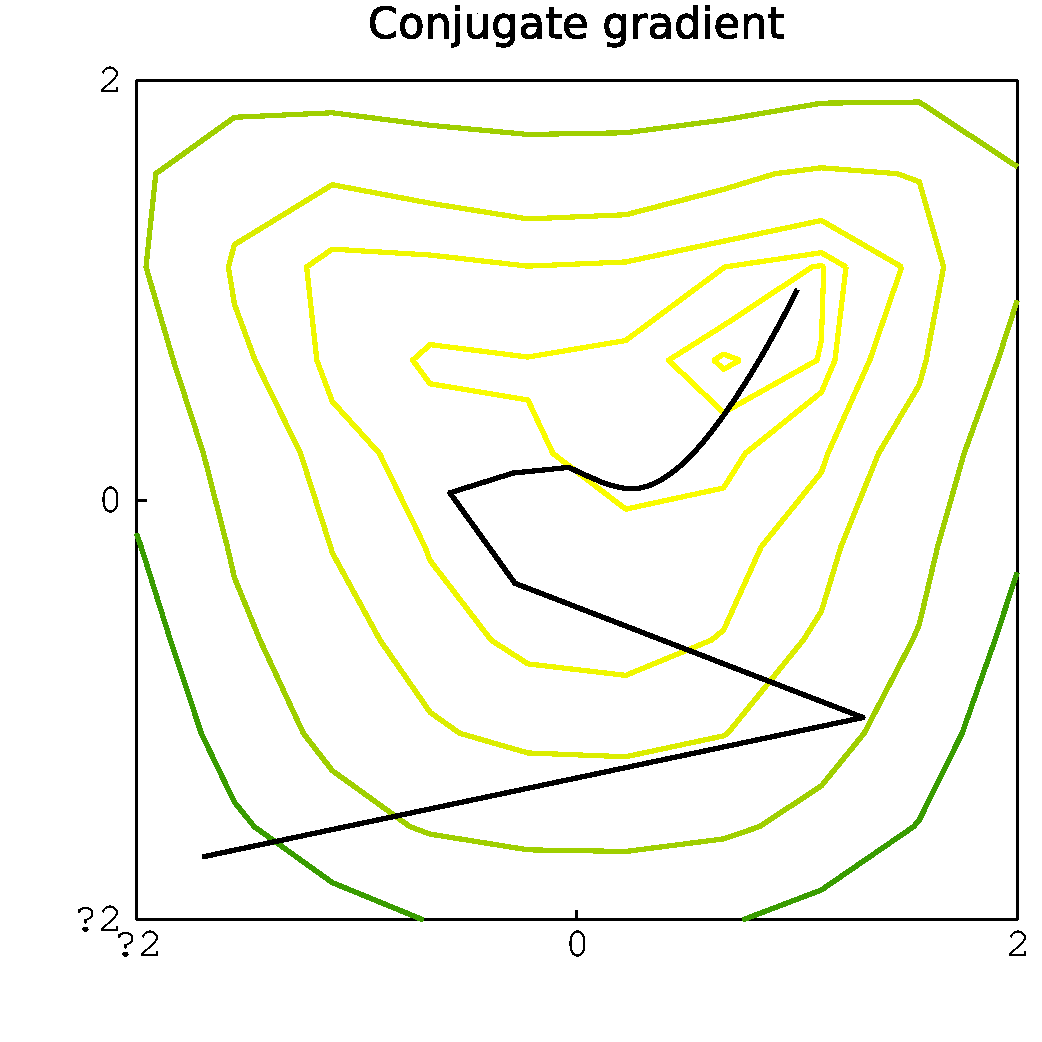
\includegraphics[width=10cm]{Figuras/Conjugate_gradient_linef1}
	\caption{Método de otimização \textit{conjugate gradient descent} para a segunda função. Utilizada a linha de busca simples.}
	\label{fig:conj1}
\end{figure} 
\begin{figure}[ht!]
	\centering
	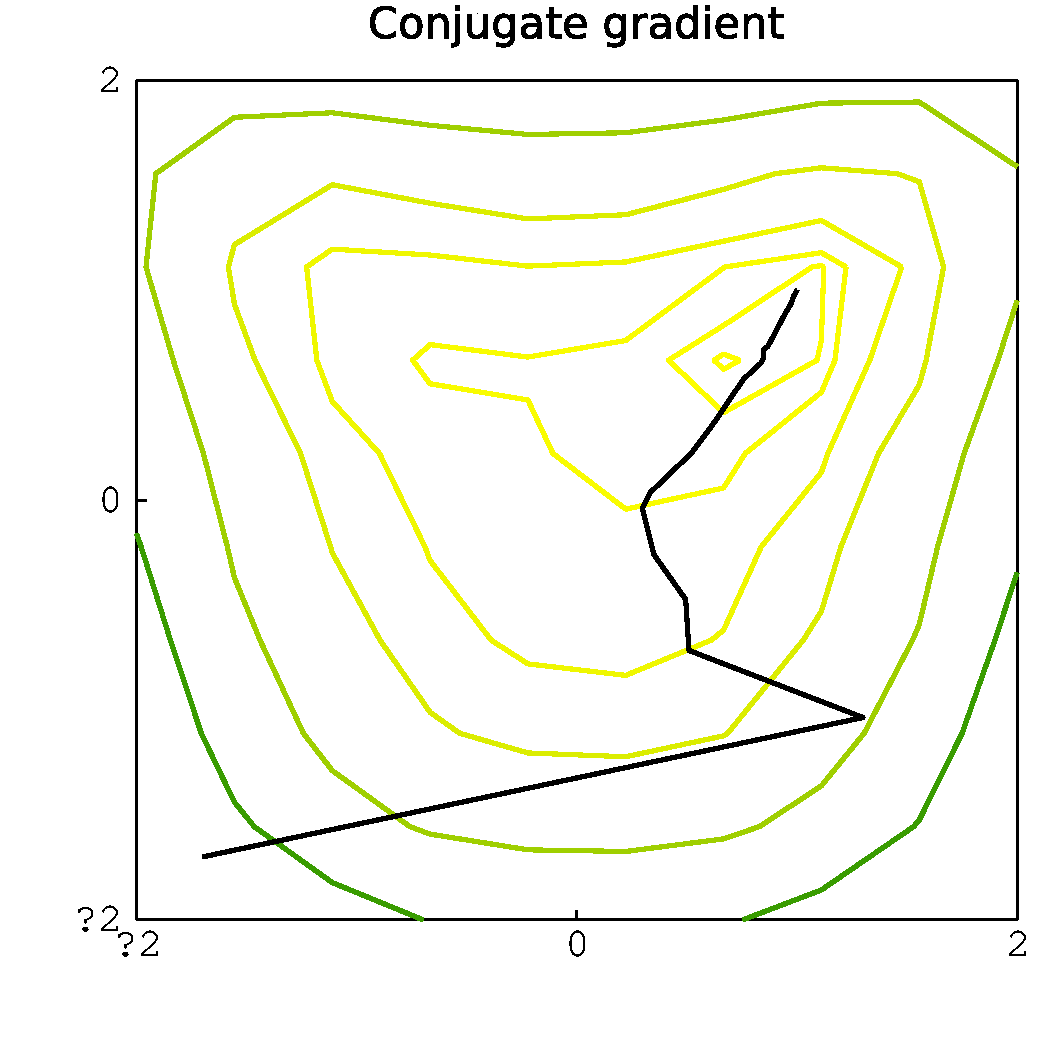
\includegraphics[width=10cm]{Figuras/Conjugate_gradient_strongf1}
	\caption{Método de otimização \textit{conjugate gradient descent} para a primeira função. Utilizada a linha de busca com as condições fortes de Wolf.} 
	\label{fig:conj3}
\end{figure} 
\subsection{MÉTODO DE SEGUNDA ORDEM}
\subsubsection{MÉTODO DE NEWTON} 
Para este método, foi colocado o máximo de 1000 iterações para avaliar as funções. Na primeira função, foram necessárias a mesma quantidade de iterações da busca simples e da condição forte de Wolf para chegar no resultado esperado, 2 iterações.
\begin{figure}[ht!]
	\centering
	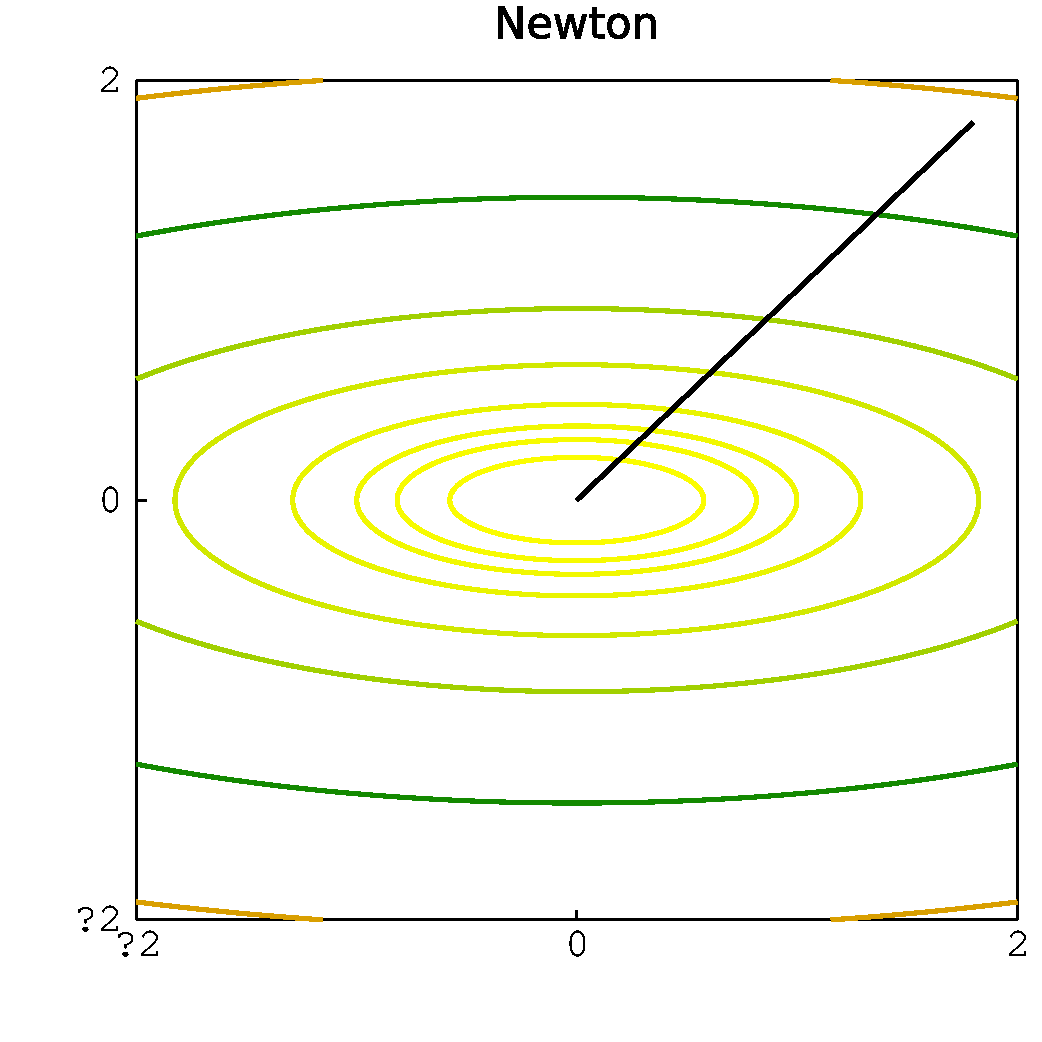
\includegraphics[width=10cm]{Figuras/Newton_linef2}
	\caption{Método de otimização de Newton para a primeira função. Utilizada a linha de busca simples.} 
	\label{fig:new1}
\end{figure} 

\begin{figure}[ht!]
	\centering
	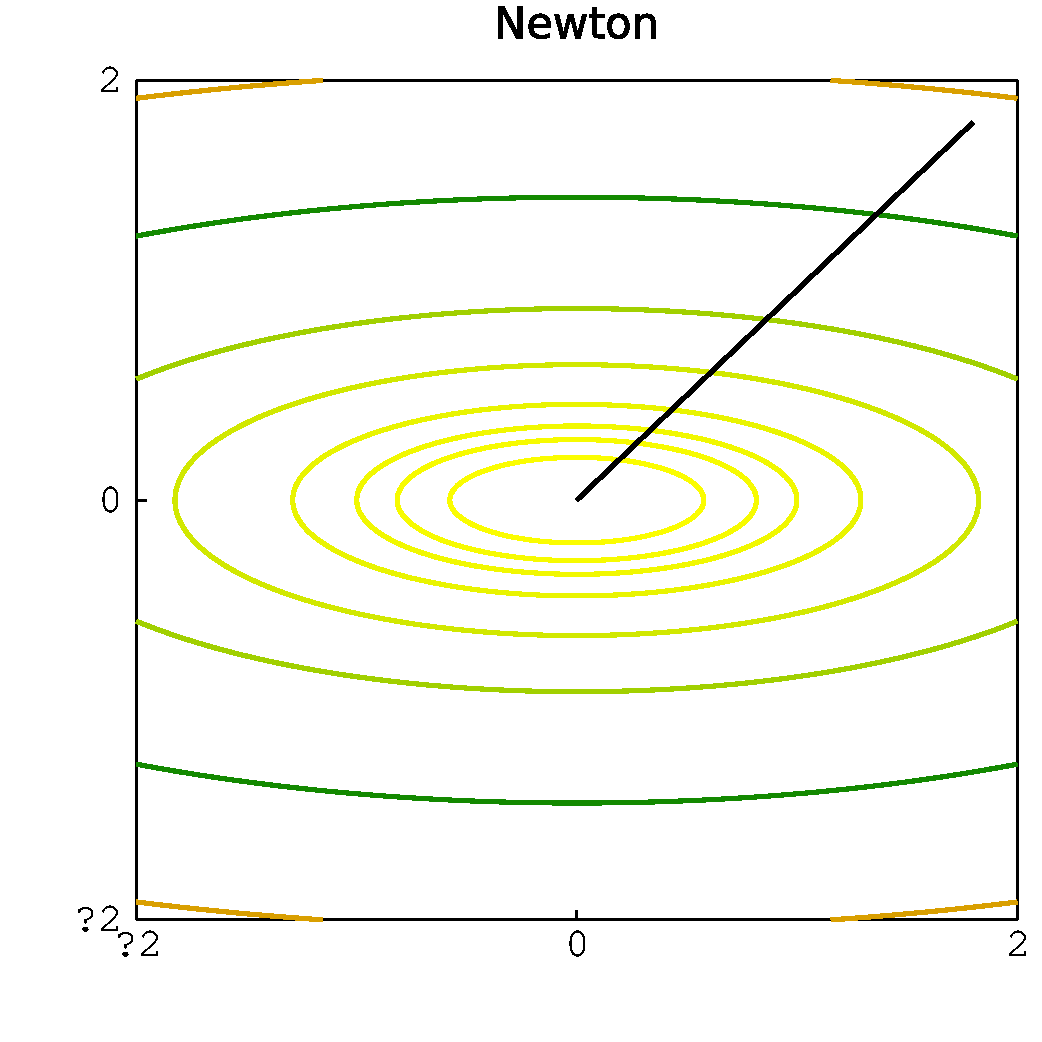
\includegraphics[width=10cm]{Figuras/Newton_wolff2}
	\caption{Método de otimização de Newton para a primeira função. Utilizada a linha de busca com condições fortes de Wolf.} 
	\label{fig:new3}
\end{figure} 
Diferente do caso anterior, as iterações variaram dependendo da busca de linha. Para a simples foram necessárias 14 iterações, enquanto para as condições fortes de Wolf foram 15.
\begin{figure}[ht!]
	\centering
	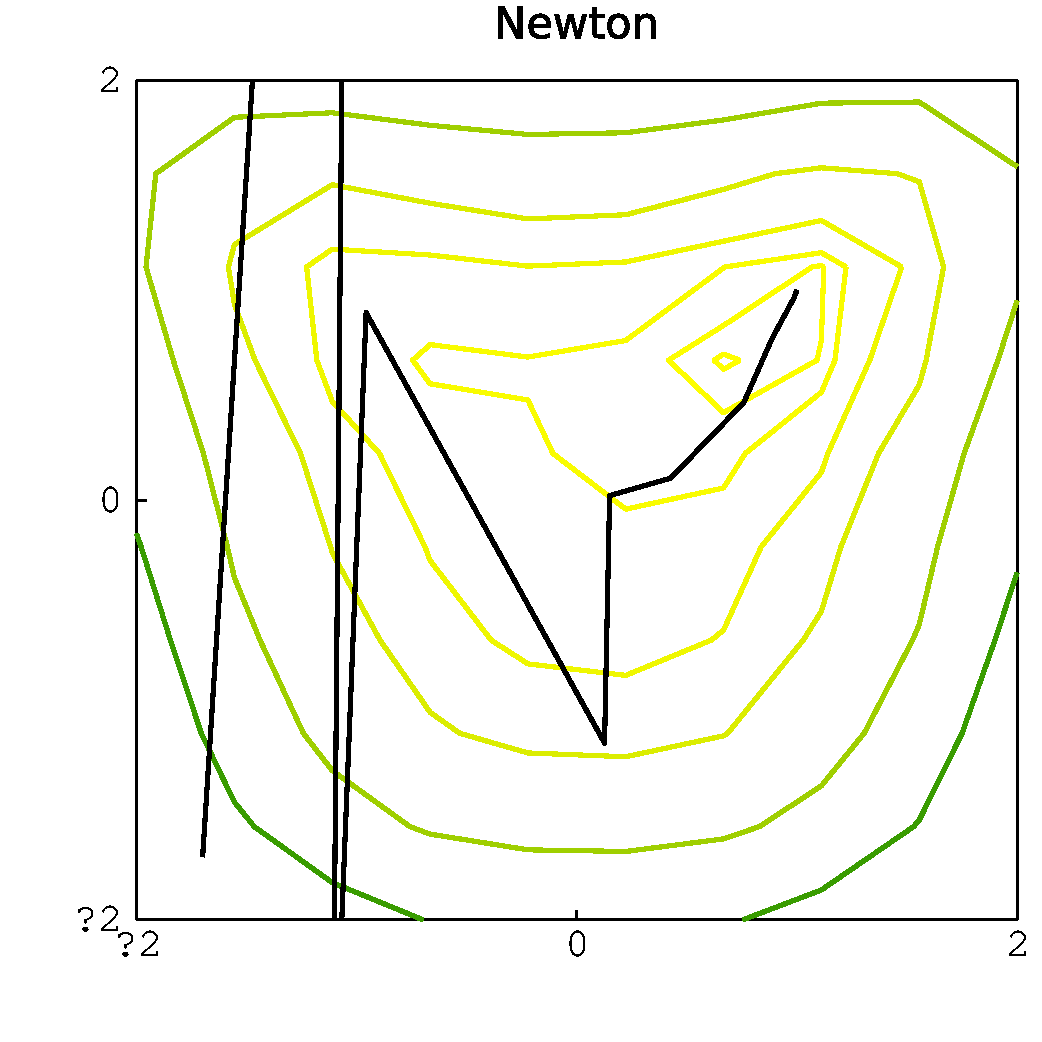
\includegraphics[width=10cm]{Figuras/Newton_linef1}
	\caption{Método de otimização de Newton para a segunda função. Utilizada a linha de busca simples.} 
	\label{fig:new1f}
\end{figure} 

\begin{figure}[ht!]
	\centering
	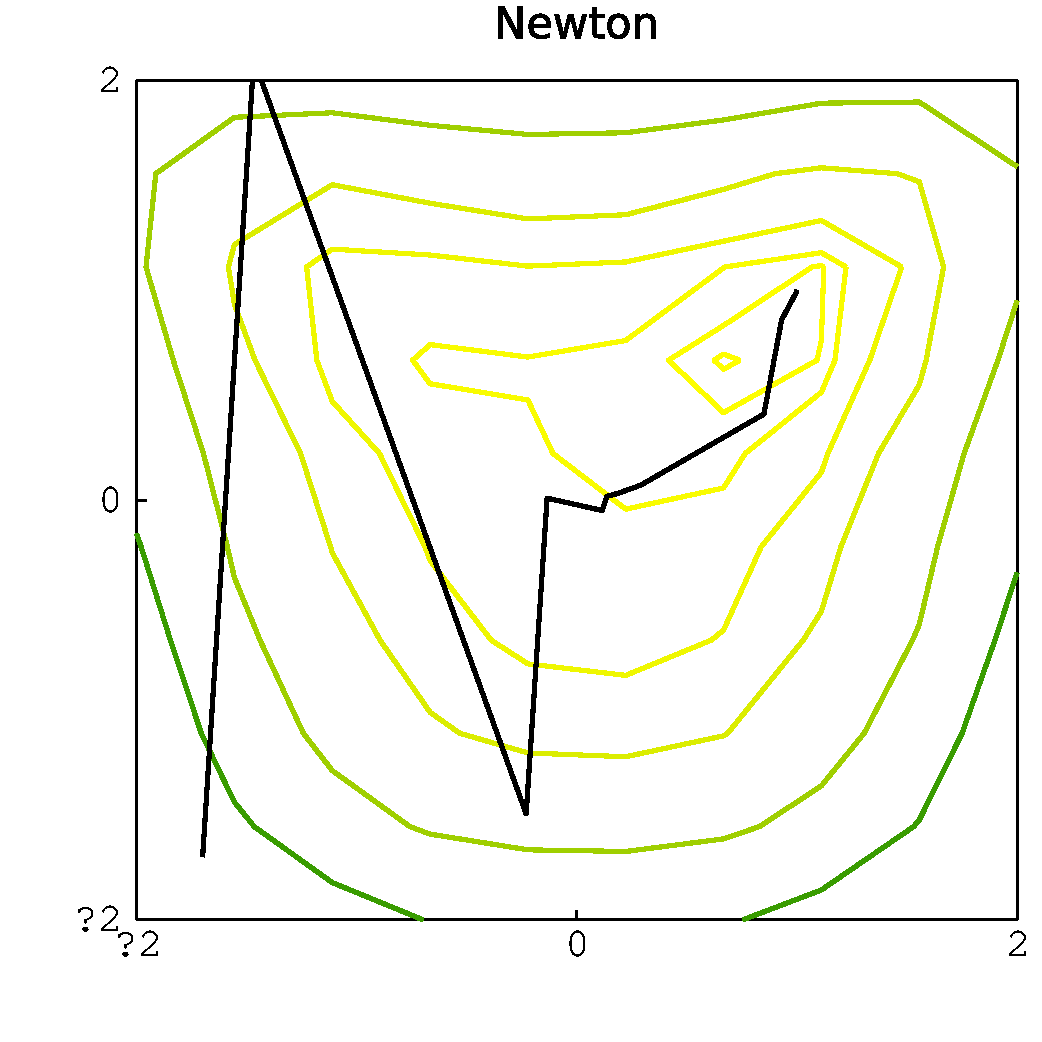
\includegraphics[width=10cm]{Figuras/Newton_strongf1}
		\caption{Método de otimização de Newton para a segunda função. Utilizada a linha de busca com condições fortes de Wolf.} 
	\label{fig:new3f}
\end{figure} 
 \section{REFERÊNCIAS BIBLIOGRÁFICAS}
 \bibliography{relatorio}
 
 
 

 \end{document}
